\documentclass[10pt,a5paper,openright]{book}

\usepackage[top=3cm,bottom=3cm,left=2.25cm,right=2.25cm,asymmetric]{geometry}
\usepackage[english]{babel}
\usepackage{subcaption}
\usepackage{graphicx} %for gnuplot with latex fonts
\usepackage{fancyhdr}
\usepackage{hyperref}
\usepackage{afterpage} %for landscape table in appendix
\usepackage{pdflscape} %for landscape table in appendix
\usepackage{changepage} %for landscape table in appendix
\usepackage{eurosym} %for euro symbol
\usepackage{cite}

\usepackage{float}

\pagestyle{fancy}
\renewcommand{\footrulewidth}{0.4pt}
\fancyhf{}
\chead{}
\fancyhead[RO]{Master in La scienza nella pratica giornalistica}
\fancyhead[LE]{Giulio Mazzolo}
\fancyfoot[C]{\thepage}

\raggedbottom

\begin{document}

 \input{Thesis_chapters/title_page}

 \newpage
 \null
 \thispagestyle{empty}
 \newpage
 
 \pagenumbering{Roman}
 
 \chapter*{Abstract}
This thesis presents an analysis of the online communication activity of EU-funded research projects in Future and Emerging Technologies (FET) within the Horizon 2020 programme. In particular, it focuses on the use of the Twitter platform by FET projects in high performance computing (HPC) and quantum technologies (QT).

FET projects were found to be present on disparate social media. More than 95\% of the projects have created a website. The most used social networks are: Twitter ($\sim 50\%$ of the projects), Facebook ($\sim 20\%$) and LinkedIn ($\sim 15\%$). Finally, the analysis suggests that the number of online channels considered by each FET project is not strongly influenced by the available budget, but rather by the pursued communication strategy.

HPC projects are among the most socially active initiatives within the FET environment. In particular, roughly 80\% of them have created a profile on Twitter. Among HPC projects, the average posting rate is of the order of one tweet per week. The Twitter activity of HPC initiatives is typically comparable to that of the FET profile in terms of \textit{i}) number of account's tweets retweeted by other users, and \textit{ii}) average number of shared links per tweet (approximately 30\% and 0.4, respectively). Currently, the most influential HPC projects on Twitter have roughly more than 100 followers and a ratio between followers and followed accounts larger than 2. Finally, conversations mentioning HPC projects were found to be extremely viral and capable of reaching hundreds of thousands of users.

Contrarily to HPC projects, no QT initiative has created an account on Twitter. An analysis was performed to estimate the potential reach of QT projects on this social platform. The investigation was based on the amount of mentions of specific hashtags. The result indicates that QT projects may reach a Twitter community comparable to that of HPC initiatives. \\

\noindent
\textbf{Key words:} science communication, high performance computing, quantum technologies, Future and Emerging Technologies, Horizon 2020, social media.
 \addcontentsline{toc}{chapter}{Abstract}
 
 \newpage
 \null
 \newpage
 
 \tableofcontents
 
 \newpage
 \null
 \newpage
 
 \pagenumbering{roman}
 %\setcounter{page}{1} 
 
 \renewcommand{\chaptermark}[1]{\markboth{#1}{}} 
 \chapter*{Synopsis}
Lorem ipsum dolor sit amet, consectetur adipisci elit, sed eiusmod tempor incidunt ut labore et dolore magna aliqua. Ut enim ad minim veniam, quis nostrum exercitationem ullam corporis suscipit laboriosam, nisi ut aliquid ex ea commodi consequatur. Quis aute iure reprehenderit in voluptate velit esse cillum dolore eu fugiat nulla pariatur. Excepteur sint obcaecat cupiditat non proident, sunt in culpa qui officia deserunt mollit anim id est laborum.

Lorem ipsum dolor sit amet, consectetur adipisci elit, sed eiusmod tempor incidunt ut labore et dolore magna aliqua. Ut enim ad minim veniam, quis nostrum exercitationem ullam corporis suscipit laboriosam, nisi ut aliquid ex ea commodi consequatur. Quis aute iure reprehenderit in voluptate velit esse cillum dolore eu fugiat nulla pariatur. Excepteur sint obcaecat cupiditat non proident, sunt in culpa qui officia deserunt mollit anim id est laborum.
 \chaptermark{Synopsis}
 \addcontentsline{toc}{chapter}{Synopsis} 
 
 \newpage
 \pagenumbering{arabic}
 \setcounter{page}{1}

 \part{Introduction}
 %\newpage
 %\null
 %\newpage

 \renewcommand{\chaptermark}[1]{\markboth{\thechapter.\ #1}{}}
 \chapter{The role of science communication} \label{The_role_of_science_communication}
This chapters presents a concise overview of the importance of science communication in modern society. Section \ref{The_knowledge_era} outlines the characteristics of the knowledge era. Section \ref{Challenges_in_the_knowledge_era} focuses on the related economical and societal challenges. Section \ref{The_scientific_citizenship} highlights the need for scientific citizenship in the knowledge era. Section \ref{Science_communication_and_modern_society} presents science communication as a requirement for the acquisition of the scientific citizenship. 

\section{The knowledge era} \label{The_knowledge_era}
Three economical eras have been identified in the history of human civilisation. The first one was the agricultural era. This is believed to have started between 10000 and 8000 B.C. in different regions in the world \cite{Bocquet,Barker}. The second one is the industrial era. It began in England in the 18th century as a result of the industrial revolution \cite{Trinder, Griffin}. The third one is the knowledge era, and it is the age into which human civilization is currently entering \cite{Bohme-Stehr}. 

The three eras are based on different primary production resources. The agricultural age was founded on the work of people and animals. The ultimate source of richness and development in the industrial era was the work of people and machines. Finally, the current era is not based on the capacity to produce and accumulate tangible goods, but rather on the ability to accumulate, generate and apply new knowledge \cite{Powell}.

The knowledge on which the current era is based is mainly scientific. In the past centuries, the impact of science on humanity has been growing without interruption \cite{Pickstone}. Nowadays, the outcomes of scientific activities permeate our society and life style. Examples range from telecommunications to medicine, or from artificial intelligence to the development of new materials.

The reason for the increasing impact of science is the peculiar nature of scientific knowledge as a resource \cite{Probst}. Like any other resource, it is important for the capacity to provide solutions to problems. However, contrarily to resources such as water, food or oil, scientific knowledge is potentially unlimited, as it is capable of generating itself (knowledge leads to new knowledge). Moreover, the same knowledge can be used simultaneously by multiple entities. Hence, scientific knowledge is intrinsically a non-exclusive good.

For its characteristics as a resource, scientific knowledge has revolutionised the world economy. The current science-driven change of the global market has introduced countless positive innovations. However, it has also led to dramatic societal changes.   

\section{Challenges in the knowledge era} \label{Challenges_in_the_knowledge_era}
The relationship between scientific research and society has \, \, changed significantly after the Second World War. From the second half of the 20th century, several countries have started using science and its generation of new knowledge and technology as a source of economical growth. This process has progressively become more intense over the last decades. Nowadays, nations invest significant fractions of their gross domestic product in research and development. Examples are the European Union, the United States, and Asiatic countries such as China and South Korea, see figure \ref{GD_investment}.    

\begin{figure}[!t] 
 \begin{center}
 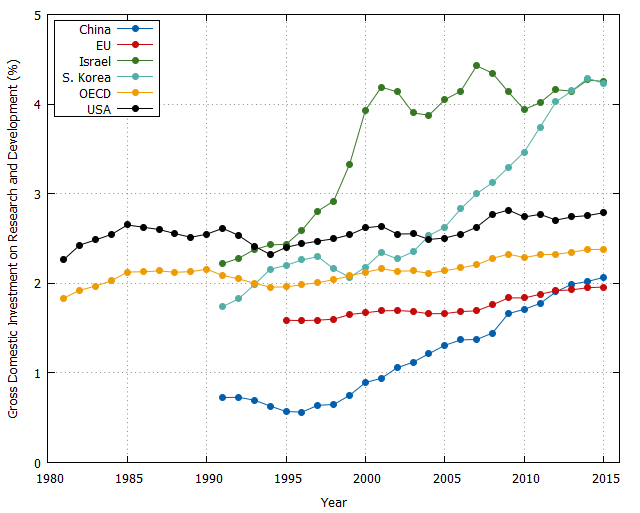
\includegraphics[scale=0.4]{Images/GD_investment.png}
 \caption{Percentage of the gross domestic product invested in science and development over the past years by some of the world's leading economies. The image is based on data of the Organisation for Economic Co-operation and Development (OECD) \cite{OECD}.}
 \label{GD_investment}
 \end{center}
\end{figure}

The capacity of scientific knowledge to generate richness has attracted a growing number of private investors. As a result, in many countries private investment on scientific research is larger than public funds \cite{UNESCO}. One example are the United States, where the former is currently twice as large as the latter \cite{Boroush}. 

\begin{figure}[!t] 
 \begin{center}
 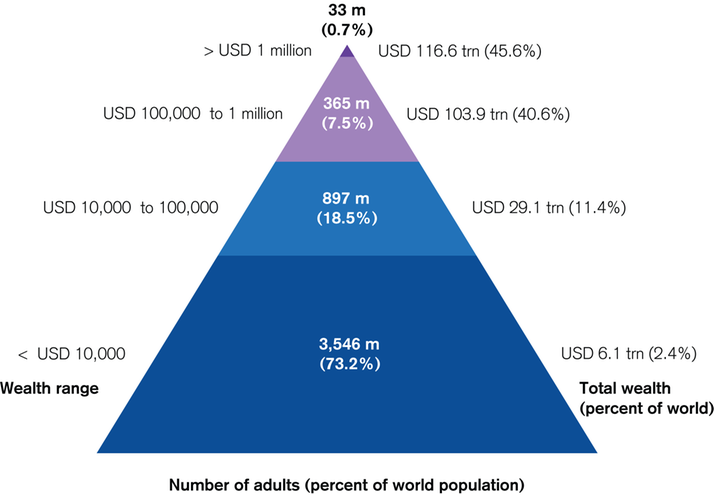
\includegraphics[scale=0.4]{Images/Global_wealth_pyramid.png}
 \caption{Distribution of the global wealth among the world's population. Original image in \cite{Kersley}.}
 \label{Global_wealth_pyramid}
 \end{center}
\end{figure}

The leading role of private investors is based on a reinterpretation of knowledge as a resource. To pursue personal profit, investors are typically non interested in sharing the knowledge they develop or they way they use it to create goods. This approach limits the possibility to generate new knowledge from the results of others. Moreover, people with limited buying power cannot afford specific classes of products and benefit from the knowledge behind them. One example are patented expensive medicines \cite{Heller}. In such a scenario, knowledge as a resource partially looses the intrinsic characteristics mentioned in Section \ref{The_knowledge_era} of being unlimited and non exclusive. 

\begin{figure}[!t] 
 \begin{center}
 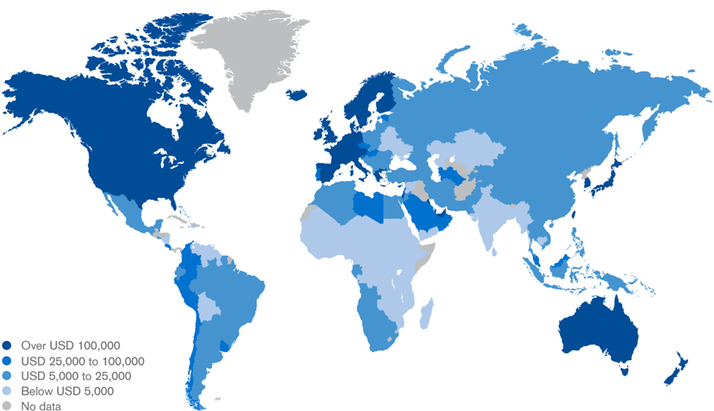
\includegraphics[scale=0.4]{Images/World_wealth_levels.png}
 \caption{Comparison among nations of the current annual wealth per adult. Original image in \cite{Kersley}.}
 \label{World_wealth_levels}
 \end{center}
\end{figure}

The current knowledge-driven development of the global economy has two important consequences. First, humanity is richer than ever before \cite{Maddison}. Second, the progressive concentration of the generated richness in the hands of few individuals is causing societal inequality, see figures \ref{Global_wealth_pyramid} and \ref{World_wealth_levels}. 

The increasing inequality is an obstacle for the creation of a democratic society \cite{Mckenna}. The scenario humanity is facing can change if knowledge will not be used as a mere instrument of power, but rather as a common good everyone should benefit from. This paradigm shift can be achieved through the acquisition of the scientific citizenship.

\section{The scientific citizenship} \label{The_scientific_citizenship}
The potential of scientific knowledge to be a pillar of democratic societies was first recognised by the English philosopher Francis Bacon in the 17th century. He proposed that science and technology should not bring advantages to a limited number of societal groups or nations, but rather to the whole humankind \cite{Zagorin}. This vision is efficaciously outlined in his utopian novel \textit{The New Atlantis}.

Bacon's ideas are extremely topical. As mentioned in section \ref{Challenges_in_the_knowledge_era}, the equal access to goods generated by scientific research is fundamental to prevent societal divisions and exclusions.

A second ingredient for the creation of a democratic society is the people's awareness of the scientific process, as well as of its goals, outcomes and limits \cite{Gibbons}. In fact, democratic societies are founded on the engagement of citizens when decisions impacting the community must be taken. Because of the permeating role of science in today's society, science-related issues are no exception \cite{vanDijck}. Examples are topics such as mandatory vaccination, euthanasia, abortion, animal experimentation, alternative medicine, nuclear energy, recycling and, in general, the public investments on research assigned by policy makers. Hence, a better understanding of science is a key factor to ensure effective participatory processes \cite{Shapin}.    

The population's engagement in decision-making processes is only fruitful if scientific innovations are neither passively accepted nor irrationally feared. To this aim, people must be given the ability to intervene in an informed, rational and critical way. This scenario is only possible if individuals are formed and trained in an adequate cultural context. In other words, if people acquire the so-called scientific citizenship \cite{Arnason}.

How to best prepare individuals to become scientific citizens is still debated \cite{Nowotny}. Nevertheless, a key ingredient has been identified in the need to bring scientists and citizens closer to each other. It is widely accepted that the construction of a democratic knowledge era depends crucially on the continuous dialogue and information and knowledge exchange between these two communities. A paradigm which motivates the growing importance of science communication.

\section{Science communication and modern society} \label{Science_communication_and_modern_society}    
Science relies heavily on communication. Research is only useful if communicated to the rest of the scientific community. This has become even more crucial in the era of Big Science \cite{Galison}. Modern physics offers illustrative examples in this direction. Large-scale experiments such as the LHC particle accelerator at CERN in Switzerland or the LIGO-Virgo gravitational-wave observatories in the USA and Italy are built and maintained by international collaborations of thousands of scientists from tens of different countries \cite{CERN, LIGO, Virgo}. These titanic efforts can only be successful if supported by effective internal communication.  

The relationship between science and communication has \, evolved with the transition to the knowledge era \cite{Holliman}. Nowadays, science communication can no longer happen exclusively within the scientific community. As outlined in Section \ref{The_scientific_citizenship}, the construction of a democratic society requires the engagement of disparate societal groups in the decision-making processes related to scientific questions \cite{Wynne}. Examples are scientists, policy makers, private investors, non-governmental organizations, the general public etc. When discussing with each other, these groups make use of science communication.

The aforementioned societal groups have different cultural background and objectives. Thus, they adopt different languages when talking about scientific issues. Moreover, to be effective, each group must tune its science communication on the targeted audience, with the optimal choice depending on both the content and the considered communication channel. As a consequence, numerous different kinds of science communication can be identified.   

This thesis focuses on science communication aiming to inform citizens on a non-technical level of current investigation lines. This is the oldest type of science communication not confined within the scientific community. The first example in this direction was the \textit{De Rerum Natura} by the Roman poet Lucretius in the first century BC. Another milestone in this direction was Galileo Galiei's \textit{Sidereus Nuncius} in the 17th century. His work spread all over the world short after publication and revolutionised humanity's self-perception by propagating the author's innovative astronomical discoveries \cite{Burke}.

More specifically, this thesis focuses on research projects funded by the European Union within the Future and Emerging Technologies programme and on their use of the web 2.0 social media to communicate results and objectives. As outlined in the next chapters, the ultimate goal is to investigate whether European scientists are properly exploiting today's most effective communication channels to inform citizens of two very important scientific challenges: high-performing computing and the development of quantum technologies.

\section{Chapter summary} 
In this chapter, the following items have been discussed:

\begin{enumerate}
 \item Human society is currently entering the so-called knowledge era. This age is characterised by the fact that scientific knowledge has become one of the most important sources of wealth. 
 \item The knowledge era offers unprecedented opportunities to improve the quality of people's life. However, it also presents new societal challenges. In particular, the unequal access to scientific knowledge and technology may prevent the realisation of democratic systems.
 \item The construction of a democratic society in the knowledge era depends on the engagement of citizens and stakeholders in the debate about the impact of scientific issues on their lives. This can be achieved by training people to discuss scientific questions in a constructive and critic way, i.e., by helping individuals acquire the so-called scientific citizenship.
 \item One key factor to help people acquire the scientific citizenship is science communication. There exist disparate kinds of science communication, depending on the interacting societal groups. The present thesis focuses on science communication conducted via social media to inform citizens of EU-funded research projects.     
\end{enumerate}
 \chapter{FET in Horizon 2020}
This chapter focuses on the FET funding programme and its research lines relevant for this thesis. Section \ref{The_Horizon_2020_programme} illustrates the Horizon 2020 initiative. Section \ref{The_FET_programme} is a description of FET in the framework of Horizon 2020 and its main calls for funding. Sections \ref{FET_and_high-performing_computing} and \ref{FET_and_quantum_technologies} summarise the FET effort towards the development of quantum technologies and high-performing computers.

\section{The Horizon 2020 programme} \label{The_Horizon_2020_programme}
Horizon 2020 is the biggest Research and Innovation programme funded by the European Union to date. It targets a smart and sustainable societal and economic growth via the development and application of scientific research. The available budget totals nearly 80 billions Euro over a seven-year period (from 2014 to 2020).

Horizon 2020 is Europe's eighth Research and Innovation programme in chronological order. The first was launched in 1984. Duration and allocated budget of each Research and Innovation programme is shown in figure \ref{FP_funds}.

\begin{figure}[!t] 
 \begin{center}
 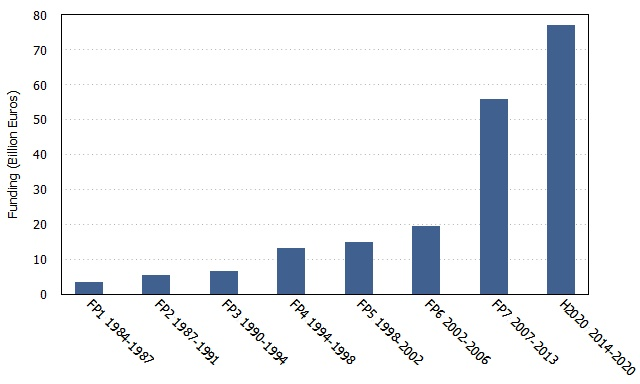
\includegraphics[scale=0.4]{Images/FP_funds.jpg}
 \caption{Duration and allocated budget of Europe's Research and Innovation programmes (also known as Framework Programme, FP). Budgets are expressed in billion Euros. Data from \cite{OECD}.}
 \label{FP_funds}
 \end{center}
\end{figure}

%data from https://ec.europa.eu/research/fp7/pdf/fp-1984-2013_en.pdf#view=fit&pagemode=none

Any natural or legal persons (e.g., universities, research organisation and companies) can apply for Horizon 2020 funding. Applications must fit into one of the following categories: 

\begin{itemize}
 \item \textbf{Excellent Science:} this initiative supports the excellence of European scientific research on a global level and in a variety of fields.
 \item \textbf{Industrial Leadership:} this class of projects targets the development of technological innovations for the future market and the growth of European small and medium enterprises.
 \item \textbf{Societal Challenges:} this group focuses on priorities of the European society such as health, education, energy supply and food by combining knowledge and methods from disparate scientific fields.  
 \item \textbf{European Institute for Innovation and Technology:} this institute is an independent European body supporting growth via the promotion of synergies in the fields of education, research and business. 
 \item \textbf{Euratom:} this pillar contributes to the decarbonisation of the energy supply through safe nuclear research.
\end{itemize}
The Horizon 2020's budget breakdown into the aforementioned lines of action is shown in figure \ref{H2020_budget_breakdown}.

\begin{figure}[!t] 
 \begin{center}
 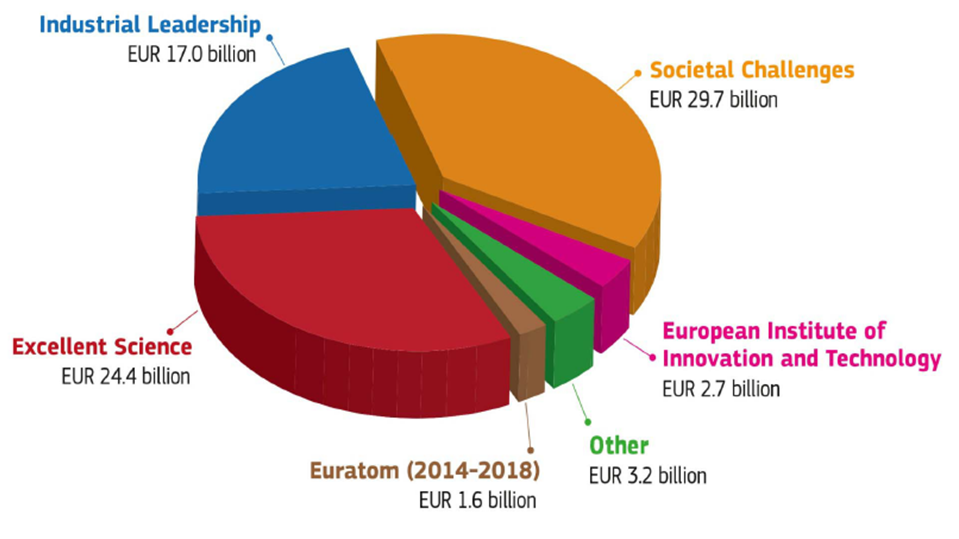
\includegraphics[scale=0.3]{Images/H2020_budget_breakdown.png}
 \caption{Budget breakdown of the Horizon 2020 programme. Original image in \cite{OECD}.}
 \label{H2020_budget_breakdown}
 \end{center}
\end{figure}

\section{The FET programme} \label{The_FET_programme}
As mentioned in section \ref{The_Horizon_2020_programme}, one of the actions of Horizon 2020 is the Excellent Science programme. This initiative supports researchers and institutions developing new science and cutting-edge technology. The goal is to keep European research at the forefront of scientific innovation and discover applications to improve the citizens' life and ensure economical growth.  

\begin{table}[t]
 \begin{center}
  \begin{tabular}{cc}
   \hline 
   \hline
   Line of action & Estimated final budget \\ 
   \hline
   \hline
   ERC & 13.1 \\
   FET & 2.7 \\
   MSCA & 6.2 \\
   RI & 2.5 \\
   \hline
   \hline
  \end{tabular}
 \end{center} 
 \caption{Estimated final budget breakdown of the Excellent Science initiative. ERC stands for European Research Council; FET for Future and Emerging Technologies; MSCA for Marie Sk\l{}odowska-Curie Actions; RI for Research infrastructure. Budgets are in billion Euros. Data from \cite{OECD}.}
\label{FET_budget_breakdown} 
\end{table}

Excellent Science is based on the following pillars: 

\begin{itemize}
 \item \textbf{European Research Council:} it distributes funding in every research field to single scientists and with the requirement of scientific excellence.  
 \item \textbf{Future and Emerging Technologies (FET):} it finances collaborative research exploring visionary and radically new investigation lines. 
 \item \textbf{Marie Sk\l{}odowska-Curie Actions:} this initiative assigns grants to researchers at any stage of their career with the goal to encourage mobility between countries and fields of expertise. 
 \item \textbf{Research infrastructure:} it promotes the creation of transnational networks of research infrastructures as well as the training of qualified staff. 
\end{itemize}
The estimated final budget breakdown of Excellent Science is reported in table \ref{FET_budget_breakdown}.

\begin{figure}[!t] 
 \begin{center}
 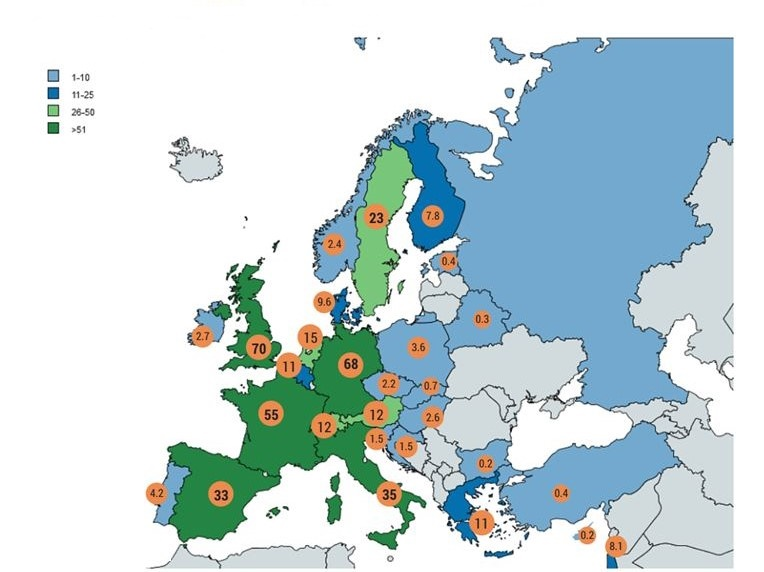
\includegraphics[scale=0.3]{Images/Country_participation_in_H2020_FET_projects.jpg}
 \caption{Participation in the Horizon 2020 FET programme on a country basis as of June 2016. Numbers correspond to FET funding in millions of euro. Colours indicate the number of participants. Adapted from image in ....}
 \label{Country_participation_in_H2020_FET_projects}
 \end{center}
\end{figure}

%image downloaded from https://ec.europa.eu/programmes/horizon2020/en/news/infographic-participation-horizon-2020-fet-projects

This thesis focuses on the communication activity of the 151 FET projects funded to date within Horizon 2020. The list of these projects is available in appendix \ref{List_of_FET_projects}. Their distribution per country as of June 2016 is shown in figure \ref{Country_participation_in_H2020_FET_projects}.

The FET funding scheme comprises three calls for applications: FET Open, FET Proactive and FET Flagship.

\subsubsection{FET Open}
The FET Open call is not bound to one specific investigation theme. However, submitted research proposals must satisfy the following ``gatekeepers": scientific and technological breakthrough; foundational; novelty; high-risk; long-term vision; interdisciplinary. 

FET Open promotes the Coordination and Support Actions (CSA) as well. These aim at identifying and fulfilling the optimal conditions for FET-related collaborative ... . One CSA type of action is FET Innovation Launchpad, which investigates and explores possible economical and societal applications of FET results. The list of Horizon 2020 projects funded within the FET Innovation Launchpad action is reported in appendix \ref{Specific_lists_of_FET_projects}. 

\subsubsection{FET Proactive}
The FET Proactive call nurtures the birth of synergies on specific research lines by bringing together scientists from interdisciplinary fields. Considered research lines are not ready for the market yet.    

Currently, FET Proactive comprises three calls related to ``Boosting emerging technologies" and three under ``High Performance Computing". Given its relevance for this thesis, the ``High Performance Computing" FET Proactive call is illustrated in section \ref{FET_and_high-performing_computing}. 

FET Proactive invests resources also on identifying investigation roadmaps, design and distribute material for educational purposes and disseminate FET results among interested stakeholders.  

\subsubsection{FET Flagship}
FET Flagships are Europe's main research efforts. They are large-scale, decade-long projects with budgets totalling one billion Euros each. The ultimate goals are to shed light on key scientific themes and apply the results to European society. To date, three FET Flagships have been approved in the Horizon 2020 programme: 

\begin{itemize}
 \item \textbf{Human Brain Project:} it targets groundbreaking steps forward in neuroscience.
 \item \textbf{Graphene:} it explores graphene's properties and possible applications.
 \item \textbf{Quantum Technologies:} it aims at developing innovative technologies based on the laws of quantum physics.
\end{itemize}
The Human Brain Project and Graphene Flagships started in April 2016. The Quantum Technologies Flagship will start running in 2018. Given its relevance for this thesis, the Quantum Technologies Flaghisp is described in section \ref{FET_and_quantum_technologies}.

\section{FET and high-performing computing} \label{FET_and_high-performing_computing}
Current and future scientific and engineering challenges require increasing levels of computational performances. The demand can be satisfied via the construction of large computer clusters and the development of suitable programming languages. The former provide higher computational power, the latter an optimal exploitation of the clusters' resources. The use of such practices is known as high-performing computing (HPC).

In terms of increasing computational power, one major HPC goal is the transition from the peta- to the exascale. This corresponds to the increase from $10^{15}$ floating point operations per second, i.e. the limit of present-day most powerful supercomputers, to $10^{18}$. The upgrade to the exascale is motivated by its major impact on all scientific fields, hence pushing forward research and the development of new technology for the next decades. 

As mentioned in section \ref{The_FET_programme}, the European HPC effort is funded within the ``High Performance Computing" FET Proactive call. This call comprises three initiatives: \textit{i}) co-design of HPC systems and applications; \textit{ii}) transition to exascale computing; and \textit{iii}) exascale HPC ecosystem development. The main goals of the three initiatives are to develop the next-generation high-performing computers towards exascale and to provide access to the resources offered by supercomputers. The list of Horizon 2020 FET projects active in the HPC is available in Appendix \ref{Specific_lists_of_FET_projects}.


\section{FET and quantum technologies} \label{FET_and_quantum_technologies}
Quantum technologies arise from applications of quantum physics. They are an important research topic on a global level for their potential to revolutionise human societies.

The so-called first quantum revolution started at the beginning of the past century with the development of quantum theory. The growing understanding of the atomic world led to the birth of new disciplines, such as informatics and microelectronics, and to the construction of countless fundamental tools and electronic devices. Examples range from computers and cameras to lasers and photocopy machines. The first quantum revolution played a key role in starting the knowledge era of human society.

It is believed that the second quantum revolution will be driven by the ability acquired by humankind to actively engineer the quantum world to its own purposes. This is expected to lead to a complete new class of technologies which would reshape our society. One example is the development of quantum computers. If successfully developed, such machines will be far more powerful than any present and future computer based on classical architectures. The urge for Europe to stay at the forefront of the second quantum revolution is outlined in the so-called Quantum Manifesto.

%citazione articolo arxiv https://arxiv.org/ftp/quant-ph/papers/0206/0206091.pdf

The development of quantum technologies is a central objective of the FET programme.  The list of Horizon 2020 FET projects in this field is reported in Appendix \ref{Specific_lists_of_FET_projects}. Their activity is supported by the ERANET Cofund in Quantum Technologies, a FET Proactive initiative fostering synergies and partnerships among researchers and other stakeholders. Finally, as mentioned in section \ref{The_FET_programme}, one dedicated flagship initiative will be launched in 2018. 

\section{Chapter summary} 
In this chapter, the following items have been discussed:

\begin{enumerate}
 \item Horizon 2020 is the largest research funding programme of the European Union. It is planned to run from 2014 to 2020 and has a total budget of nearly 80 billion Euros. 
 \item One funding scheme of Horizon 2020 is Future and Emerging Technologies (FET). The FET call finances visionary research projects targeting scientific breakthroughs and the development and application of radically new technologies. The estimated FET final budget will total nearly 3 billion Euros. 
 \item The development of quantum technologies is part of the FET effort. In particular, a FET Flagship on quantum technologies has been approved in 2016 by the European Commission and will start in 2018. Allocated funds sum up to one billion Euros. 
 \item Another major goal of the FET initiative is the development of high-performing computers. The main focus of this investigation line is a power increase of modern supercomputers of three orders of magnitude (from $10^{15}$ to $10^{18}$ floating point operations per second). The upgrade from the peta- to the exascale will provide unprecedented computational resources in practically all scientific fields.    
\end{enumerate}
 
 \part{Analysis and results}
 
 \chapter{FET projects and social media}
This chapter presents an overview of the presence of FET projects on social media. Ut enim ad minim veniam, quis nostrum exercitationem ullam corporis suscipit laboriosam, nisi ut aliquid ex ea commodi consequatur. Quis aute iure reprehenderit in voluptate velit esse cillum dolore eu fugiat nulla pariatur. Excepteur sint obcaecat cupiditat non proident, sunt in culpa qui officia deserunt mollit anim id est laborum.

\section{Analysed FET projects} \label{Data_set}
This thesis focuses on the online communication activity of FET projects funded within Horizon 2020. The list of such projects was downloaded on 15th July 2017 from CORDIS, the main portal of the European Commission on results of EU-funded research projects. It consists of 151 projects and it is reported in Appendix \ref{List_of_FET_projects}. For each project, Appendix \ref{List_of_FET_projects} reports information on budget and start and end date, as well as the activated online communication channels. FET projects approved after 15th July 2017 are not considered in this thesis.  

Some of the projects in the list were not considered for this work. Excluded groups were the Flagship and Launchpad projects (see section \ref{The_FET_programme} for a brief description of the two groups), which were not considered representative of FET initiatives in terms of communication effort, as well as projects started after 1st February 2017. The lists of the excluded projects are reported in Appendix \ref{Specific_lists_of_FET_projects}. This procedure reduced the number of samples in the data set from 151 to 130.

Flagship projects were disregarded due to their budget.  As the available funding is far superior compared to the other FET projects, the Human Brain Project and the Graphene Flagships can invest larger resources on the communication activity. Thus, the two initiatives are outliers in the considered data set. 

Launchpad projects were not considered for this thesis as their ultimate goal is finding applications of results achieved by other FET projects and have limited interest in communication activity. Moreover, the available budget is relatively small. 

Finally, projects started after 1st February 2017 were disregarded as the time span between this date and the list download was judged insufficient to fully develop and launch an adequate communication activity. The only exception is the DEEP-EST project. In fact, by the time of writing DEEP-EST has already started its online communication activity.    

For some of the analyses in this thesis, the data set of 130 projects was divided into three sub-groups.  The first group consists of the 23 projects active in HPC and the transition to the exascale (see section \ref{FET_and_high-performing_computing}). The second subgroup includes the 12 projects in the field of quantum technologies (see section \ref{FET_and_quantum_technologies}). The third group comprises the other 95 projects. The lists of projects in the HPC and quantum technologies groups are reported in Appendix \ref{Specific_lists_of_FET_projects}. 

\section{Considered communication channels} \label{Considered_channels}
There exist disparate channels suitable for communication purposes. Those offering the widest audience are based on the internet. Examples are websites and social media. For this reason, FET projects consider the resources provided by the web as some of the main pillars of their communication strategy.

Different approaches can be considered to assess the use of online communication channels made by FET projects. One quantitative estimate is the fraction of projects active on specific platforms. For this thesis, the following communication channels were considered:   

\begin{description}
 \item [Website] The website is the online channel offering the highest degree of freedom to the owner. It allows the owner to personalise the content, the content's presentation strategy and the graphic visualisation.
 \item [Facebook] Facebook is the most used social media worldwide. It offers direct interaction among users and it is mainly designed for free time.  
 \item [Twitter] Twitter is very effective for concise science-related communication. It requires high posting rates and offers less personal interaction compared to Facebook.
 \item [Linkedin] Linkedin is ideal for professional content and enables the creation of closed groups. Nevertheless, interaction among users and outreach within the groups are limited.
 \item [YouTube] YouTube is the world's main platform for video sharing. It offers a very direct communication channel with effective monitoring tools. On the other hand, it is not very effective at engaging users and finding appropriate content may not be straightforward.
 \item [Instagram] Instagram has a very active and rapidly growing community. Effective communication via this channel requires pictures with strong visual content. Instagram offers limited interaction among users.
 \item [ResearchGate] ResearchGate offers the possibility to share technical documentation and engage in scientific discussions with researchers. As members are mainly scientists, the reachable community is significantly smaller and more homogeneous compared to other social networks.  
\end{description}

\section{Search for activated accounts}
The analyses presented in this thesis are based on the number of FET projects considering the online communication tools mentioned in section \ref{Considered_channels}. To this aim, a dedicated search was performed for all projects in Appendix \ref{List_of_FET_projects}. 

The search was conducted as follows. First, projects were contacted directly to ensure that the related information on the considered communication channels was complete. However, in some cases it was not possible to find the contact details of the project or no answer was received (dare numero). When this occurred, a desk search was performed to gather the required information. It cannot be excluded that the desk search failed to find the website or all accounts activated on the social channels considered for this thesis. Thus, it is highly probable that the list of accounts in Appendix \ref{List_of_FET_projects} is incomplete. The results presented in this thesis must therefore be considered as inferior limits when investigating the actual situation. 

\section{Overall presence} \label{Overall_presence}
Out of the 130 projects in the data set, ... have created a website, whereas ... have opened accounts on Twitter, ... on Facebook, ... on  Linkedin, ... on YouTube, ... on ResearchGate and ... on Instagram. The results, expressed in percentage, are shown in Figure \ref{Social_media}.

The results show that almost all FET projects have created a website. Facebook and Twitter are the two most popular social media within the FET community, hence reflecting the situation experienced in society. Nevertheless, the fraction of projects active on Twitter is significantly larger than that on Facebook. This is opposite to what occurs in society, where Facebook is the most used social media. This indicate that Twitter is considered a more suitable tool for scientific communication. 

\begin{figure}[!t] 
 \begin{center}
 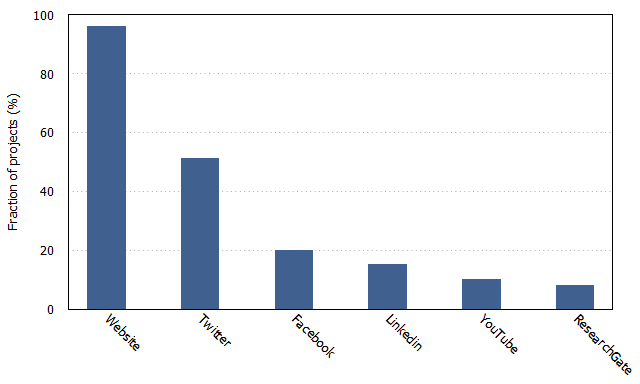
\includegraphics[scale=0.4]{Images/Social_media.png}
 \caption{Percentage of FET projects making use of the communication channels considered for this thesis.}
 \label{Social_media}
 \end{center}
\end{figure}

YouTube and Instagram are not common communication channels among FET projects. This is probably due to the difficulty of collecting visually impacting material capable of drawing attention of disparate audiences not familiar with the research field. The difficulty arises from the fact that the objectives and results of FET projects are often very technical and not appropriate for visual communication. In the case of YouTube, there is the additional problem of the high resources needed for the production of high-quality videos.

The number of projects active on ResearchGate is low. This is probably due to the fact that ResearchGate is not a suitable channel for large-scale communication activity. In fact, the reachable audience is typically limited to researchers active in similar investigation fields

\section{Presence breakdown}
The analysis in section \ref{Overall_presence} was repeated on the projects subgroups outlined in section \ref{Data_set}: HPC, QT and the others. This enable a comparison of how disparate classes of FET projects make use of online communication channels. The comparison among the three groups is shown in figure \ref{Social_media_breakdown}. 

The figure shows that websites are pillars of the communication strategies pursued by FET projects regardless of the subgroup. As for the most used social media within the FET community, i.e. Twitter, Facebook and Linkedin, the HPC subgroup has activated the most accounts compared to QT and other projects. The result indicates that HPC projects are among the most active FET initiatives in terms of online communication.  

QT projects seem to follow the opposite strategy. The number of projects making use of social media for their communication campaigns. is significantly smaller compared to HPC and other FET projects. In particular, none of them has activated an account on Twitter, the most used social platform in the FET community. 

The very limited use of social media made by QT projects highlights two facts. First, the online communication activity the QT Flagship will pursue will be designed without guidelines based on previous experiences from the same investigation field. Second, classes of projects facing similar challenges in terms of results communication and engagement of non-expert audiences may opt for very different strategies. This is the case of HPC and QT projects, as both pursue very technical goals which may look detached from society to the laymen. Moreover, the two classes target the common objective of improving current computers\footnote{Although HPC and QT projects focus on the development of present-day computers, the adopted strategies are very different: the former group aims at improving current classical architectures, the latter at exploiting a completely new approach, see sections \ref{FET_and_high-performing_computing} and \ref{FET_and_quantum_technologies}.}.

\begin{figure}[!t] 
 \begin{center}
 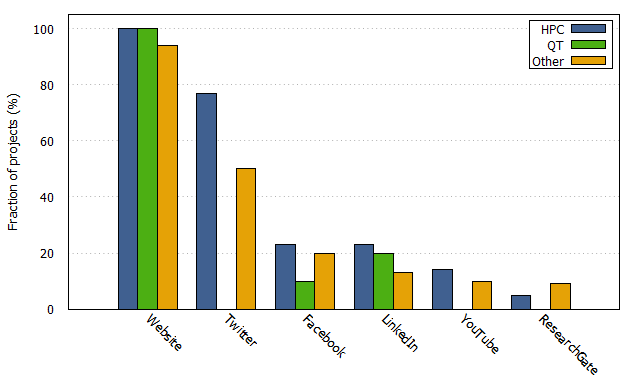
\includegraphics[scale=0.4]{Images/Social_media_breakdown.png}
 \caption{Percentage of FET projects making use of the communication channels considered for this thesis.}
 \label{Social_media_breakdown}
 \end{center}
\end{figure}

It must be beared in mind that the results presented in this section have been calculated on small data sets. The HPC and QT subgroups include ... and ... projects respectively, see Appendix \ref{Specific_lists_of_FET_projects}. The low number of projects indicates that results show limited robustness under even small changes in the data sets. The same applies to the percentages reported in figure \ref{Social_media_breakdown}. For example, the activation of a Twitter account from one single QT project would be sufficient to introduce significant variation of the result. Hence, the results reported in this section should rather serve as a guideline, and not as strong conclusions. 
 \chapter{HPC projects on Twitter} \label{HPC_projects_on_Twitter}
As shown in section \ref{Online_presence_breakdown}, roughly 80\% of the FET HPC projects have created a profile on Twitter. This percentage is larger than the corresponding value calculated for the other FET projects. Nevertheless, it is insufficient to determine whether HPC projects are conducting active communication campaigns on Twitter. 

To assess the activity and influence of HPC projects on Twitter, an analysis of their profiles was performed. The results were integrated by the monitoring activity of the mentions to HPC projects on Twitter over a period of three and a half months. The goal of this second analysis was to assess the virality of tweets on the considered projects.  

Both analyses are described in this chapter. Section \ref{Overall_activity} provides an overview of the past activity of the HPC Twitter profiles. Section \ref{Most_influential_projects} identifies the most influential HPC projects. Section \ref{Mentions_of_HPC_profiles} presents the monitoring of the mentions to HPC projects. Section ... ranks HPC project in order of virality of their mentions. 

\section{Overall activity} \label{Overall_activity}
\afterpage{
 \clearpage %Flush earlier floats (otherwise order might not be correct)
 \thispagestyle{empty} %empty page style
   \begin{landscape}
   %\begin{table}[htb]
   \begin{table}
   \begin{adjustwidth}{-1.5cm}{}
   {\tiny
    \begin{tabular}{*{8}{c}} 
      \hline 
  	  \hline
       Project & Date of first tweet & Tweets & Tweets per day & Tweets retweeted & Times per retweeted tweet & Links per tweet & Hashtags per tweet \\ 
       \hline
       \hline
       ALLScale & 26/05/2016 & 39 & 0.08 & 15\% & 1.67 & 0.72 & 0.38 \\
       ANTAREX & 25/09/2015 & 24 & 0.03 & 37\% & 1.56 & 0.63 & 0.04 \\
       COMPAT & 01/10/2015 & 122 & 0.16 & 7\% & 1.63 & 0.30 & 0.05 \\
       DEEP-EST & 19/05/2014 & 900 & 0.72 & 40\% & 2.08 & 0.52 & 1.59 \\
       ECOSCALE & 17/10/2015 & 19 & 0.03 & 21\% & 1.25 & 0.26 & 0.00 \\
       EuroLab-4-HPC & - & 0 & 0 & 0\% & 0 & 0 & 0 \\
       ExaFLOW & 27/10/2015 & 389 & 0.54 & 24\% & 1.63 & 0.62 & 0.97 \\
       ExaNeSt & 29/11/2015 & 1 059 & 1.54 & 12.5\% & 1.38 & 0.46 & 0.06 \\
       ExaNoDe & 20/06/2017 & 38 & 0.32 & 13.2\% & 2.60 & 0.21 & 0.03 \\
       EXDCI & 30/03/2016 & 864 & 1.53 & 16\% & 2.90 & 0.20 & 0.23 \\
       EXTRA & 06/10/2015 & 4 & 0.01 & 0\% & 0 & 0.25 & 0.25 \\
       INTERTWINE & 28/11/2016 & 99 & 0.31 & 51.5\% & 2.18 & 0.77 & 0.79 \\
       MANGO & 03/12/2015 & 32 & 0.05 & 43.8\% & 1.93 & 0.38 & 0.38 \\
       Mont-Blanc 3 & 06/02/2012 & 2 506 & 1.21 & 23.6\% & 2.68 & 0.32 & 0.50 \\
       NEXTGenIO & 30/09/2015 & 211 & 0.28 & 23.7\% & 3.02 & 0.14 & 0.52 \\
       READEX & 13/10/2015 & 29 & 0.04 & 69.0\% & 1.60 & 0.62 & 1.03 \\
       SAGE & 30/09/2015 & 92 & 0.12 & 32.6\% & 1.77 & 0.20 & 0.07 \\ 
       FET & 07/01/2016 & 3 199 & 4.94 & 32.3\% & 4.46 & 0.42 & 0.92 \\
       \hline
       \hline
    \end{tabular}
   }     
   \caption{Statistics collected from the Twitter accounts of the HPC projects. The data were collected from the date of the project's first tweet to 14th October 2017. Tweets per day is the average number of tweets posted each day. Tweets retweeted corresponds to the fraction of the project's tweets which have been retweeted by other accounts. Times per retweeted tweet refers to the average number of times a retweeted post has been retweeted. The last two columns report the average number of links and hashtags per project's tweet. The EuroLab-4-HPC project has posted no tweets since the creation of the account. The last row refers to the @fet\textunderscore eu profile of the FET funding programme. For this account, the statistics are limited to the maximum number of past tweets returned by Twitter (3200). The data were collected with the Twitter Analytics Tool Twitonomy.} \label{HPC_Twitter_activity}
   \end{adjustwidth} 
   \end{table}
   \end{landscape}
 \clearpage
}

The past activity of the Twitter accounts of HPC projects was investigated with the Twitter Analytics Tool Twitonomy \cite{Twitonomy}. Analysed data cover the profiles' histories since their creation and till 14th October 2017. The statistics collected for each project are listed in table \ref{HPC_Twitter_activity}. The results calculated from these data are outlined in the following subsections.

\begin{figure}
 \centering
 \begin{subfigure}[t]{0.9\textwidth}
   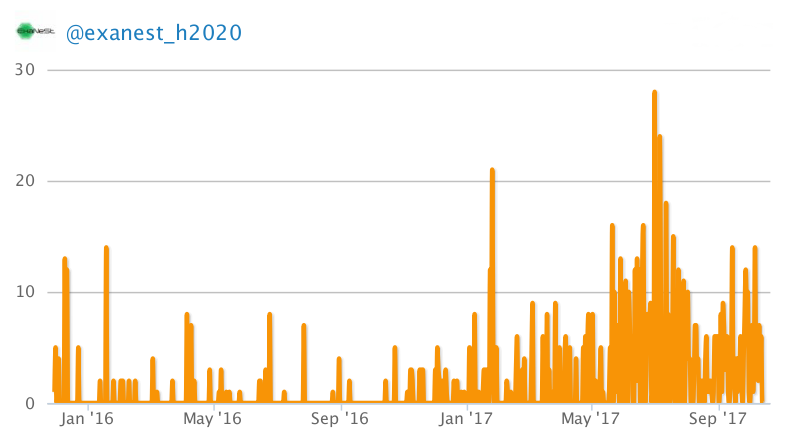
\includegraphics[width=1\linewidth]{Images/Tweets_Exanest.png}
   \caption{} 
 \end{subfigure}

 \begin{subfigure}[t]{0.9\textwidth}
   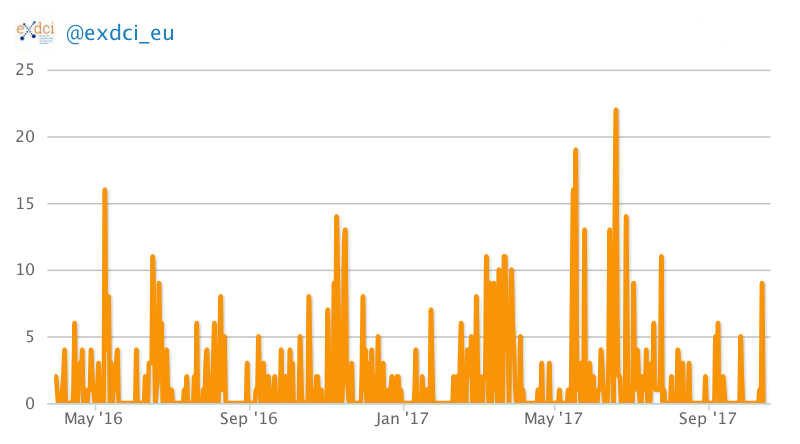
\includegraphics[width=1\linewidth]{Images/Tweets_Exdci.png}
   \caption{}
 \end{subfigure}
 \caption{(a) Time distribution of the number of tweets posted by ExaNeSt, the HPC project with the largest average number of tweets per day (1.54) as of 14th October 2017. (b) As for (a) but for EXDCI, the HPC project with the second largest average number of tweets per day (1.53). The plots were generated with the Twitter Analytics Tool Twitonomy.} 
 \label{Tweets_Exanest-Exdci}
\end{figure}

\begin{figure}
 \centering
 \begin{subfigure}[t]{0.9\textwidth}
   \includegraphics[width=1\linewidth]{Images/Tweets_Montblanc.png}
   \caption{} 
 \end{subfigure}

 \begin{subfigure}[t]{0.9\textwidth}
   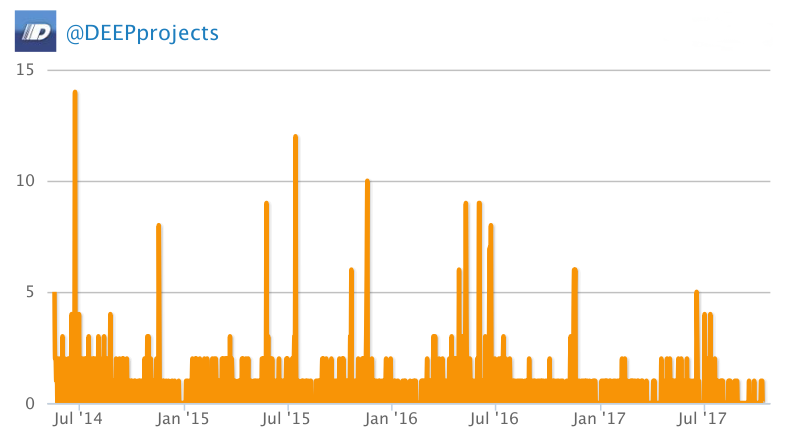
\includegraphics[width=1\linewidth]{Images/Tweets_Deepest.png}
   \caption{}
 \end{subfigure}
 \caption{(a) Time distribution of the number of tweets posted by Mont-Blanc 3, the HPC project with the third largest average number of tweets per day (1.21) as of 14th October 2017. (b) As for (a) but for DEEP-EST, the HPC project with the fourth largest average number of tweets per day (900). The plots were generated with the Twitter Analytics Tool Twitonomy.} 
 \label{Tweets_Montblanc-Deepest}
\end{figure}

\subsubsection{Tweets per day}
Out of the seventeen considered HPC projects, three have an average tweeting rate larger than one post per day. The time distribution of the tweets of the accounts with the highest average rates are shown in figures \ref{Tweets_Exanest-Exdci} and \ref{Tweets_Montblanc-Deepest}. The tweeting rate is lower than once every second day for twelve profiles. In particular, one project has posted no tweets since the creation of the account. 

The median of the projects' rates is 0.16 tweets/day. This corresponds to roughly 5 posts per month. The median was chosen as representative value of the HPC posting rates for its robustness in the presence of outliers, see also section \ref{Budget_impact}.

\subsubsection{Retweets}
The percentage of an account's tweets retweeted by other users offers an estimate of the effectiveness of its activity on Twitter. The higher the percentage, the more the account is considered a valuable source of information by the Twitter community. 

The HPC project with the largest fraction of tweets retweeted by other accounts is READEX (roughly 70\%). Except for one, all other profiles have a percentage value smaller than 50\%. The median of the fraction of retweeted tweets calculated over all HPC projects is 23.6\%.

The results on the percentage of retweeted posts is integrated by the average number of times such tweets were retweeted by different users. The higher this value, the more the Twitter community finds the profile's tweets worth to be forwarded. Table \ref{HPC_Twitter_activity} shows that six projects have an average number of times of retweet higher or equal to two. The result indicates that posts are typically retweeted by more than one user. The median calculated over all profiles is 1.67.

\subsubsection{Links and hashtags}
Links and hashtags are effective ways to enhance the relevance of a Tweet. In particular, the higher the average number of links per tweet for a given profile, the more likely the account is a source of information to other users. The higher the average number of hashtags per tweet, the higher the chance that the profile's tweets are found in a search.

As shown in table \ref{HPC_Twitter_activity}, six HPC accounts have an average number of links per tweets higher or equal to 0.5. This corresponds to one link every second tweet. The median calculated over all HPC Twitter accounts is 0.32, i.e. one link every third tweet. Three projects have accounts with an average number of hashtags equal or larger than one. The median is 0.25, which corresponds to one hashtag every fourth tweet.

\subsubsection{Comparison to the FET Twitter profile}
Table \ref{HPC_Twitter_activity} reports the statistics calculated for the Twitter profile @fet\textunderscore eu of the FET funding programme as well. Data were collected starting from 7th January 2016. The date was determined by the maximum number of past tweets returned by Twitter (3200). 

The corresponding average number of tweets per day is roughly thirty times larger than the median of HPC projects. This is probably due to the largest resources available to the FET initiative compared to single HPC projects. Nevertheless, the fraction of retweeted tweets is not significantly larger than the median calculated for HPC (32\% vs 23.6\%). The same holds for the average number of links per tweets (0.42 vs 0.32), whereas the average number of hashtags is roughly four times larger (0.92 vs 0.25).

\section{Most influential projects} \label{Most_influential_projects}
There are disparate ways to estimate the influence of Twitter profiles. One is based on both \textit{i}) the number of followers, and \textit{ii}) the ratio between the number of followers and the number of accounts followed by the considered profile (following). Influential users are identified by a large community of followers and a high ratio followers/following.

\begin{table}[t]
 \begin{center}
 {\scriptsize
  \begin{tabular}{cccc}
   \hline 
   \hline
   Project & Followers & Following & Followers/Following \\ 
   \hline
   \hline
   ALLScale & 41 & 28 & 1.46 \\
   ANTAREX & 77 & 13 & 5.92 \\
   COMPAT & 131 & 160 & 0.82 \\
   DEEP-EST & 697 & 534 & 1.31 \\
   ECOSCALE & 42 & 1 & 42 \\
   EuroLab-4-HPC & 24 & 2 & 12 \\
   ExaFLOW & 206 & 90 & 2.29 \\
   ExaNeSt & 211 & 261 & 0.81  \\
   ExaNoDe & 52 & 54 & 0.96 \\
   EXDCI & 405 & 169 & 2.40 \\
   EXTRA & 45 & 18 & 2.50\\
   INTERTWINE & 106 & 59 & 1.80 \\
   MANGO & 74 & 46 & 1.61 \\
   Mont-Blanc 3 & 1 420 & 687 & 2.07 \\
   NEXTGenIO & 162 & 44 & 3.86 \\
   READEX & 116 & 55 & 2.11 \\
   SAGE & 122 & 86 & 1.42 \\ 
   FET & 6 499 & 1 612 & 4.03 \\
   \hline
   \hline
  \end{tabular}
 } 
 \end{center} 
 \caption{Number of followers and followed accounts (following) on Twitter for the HPC projects as of 14th October 2017. Influential profiles are identified by high numbers of followers and high values of the ratio between followers and following. Data were collected with the Twitter Analytics Tool Twitonomy.}
\label{HPC_influence_table} 
\end{table}

Table \ref{HPC_influence_table} lists the number of followers and of following for each HPC project, together with the ratio followers/following. Data were collected on 4th October 2017 with the Twitonomy application. The medians of the number of followers and of the values followers/following are equal to 116 and 2.07, respectively. 

\begin{figure}[!t] 
 \begin{center}
 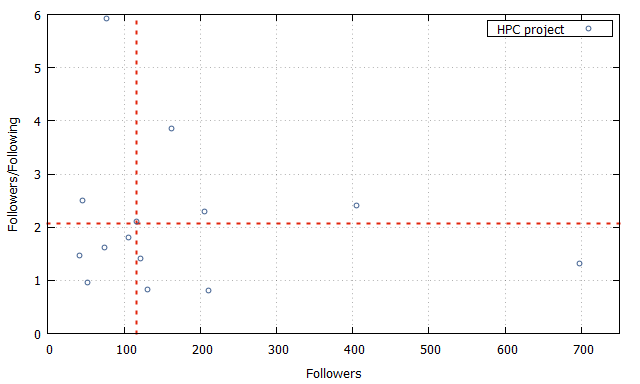
\includegraphics[scale=0.4]{Images/HPC_influence.png}
 \caption{Distribution of HPC projects as a function of the number of followers and of the ratio between followers and followed accounts (following) on Twitter. The data used for the plot were collected on 14th October 2017 with the Twitter Analytics Tool Twitonomy. The dashed lines identify the medians of the number of followers and of the values of the ratio followers/following calculated over the HPC profiles. The most influential projects are located in the upper right quarter (high number of followers and high values of followers/following). For the sake of clarity, the figure shows the follower follower/following ranges up to 750 and 6, respectively. The following projects were used to calculated the medians but lie outside the plotted ranges: ECOSCALE (42 followers, follower/following equal to 42), EuroLab-4-HPC (24 followers, follower/following equal to 12) and Mont-Blanc 3 (1420 followers, follower/following equal to 2.07).}
 \label{HPC_influence_plot}
 \end{center}
\end{figure}

To identify the most influential profiles among HPC projects, the following analysis was performed. First, projects were distributed on a plane as a function of the number of followers and of the ratio followers/following, see figure \ref{HPC_influence_plot}. Second, the plane was divided into four regions by drawing the lines corresponding to the aforementioned medians of the number of followers and of the values followers/following. The most influential HPC projects fall in the quarter of the plane identified by the conditions that the number of followers is larger than 116 and the ratio followers/following is larger than 2.07.

By following this procedure, the most influential projects are ExaFLOW (206, 2.29), EXDCI (405, 2.40), Mont-Blanc 3 (1420, 2.07) and NEXTGenIO (162, 3.86). The READEX profile (116, 2.11) is representative of the influence of HPC projects, as its values lie very close to the calculated medians.

\section{Mentions of HPC profiles} \label{Mentions_of_HPC_profiles} 
Another approach to estimate the influence of HPC projects on Twitter consists of monitoring the mentions of their accounts (i.e., @AllScaleEurope, @antarex\textunderscore project, @compatproject etc.). The monitoring activity covered the time period from 1st July to 12th October 2017 and was performed with the Twitter Analytics Tool NUVI \cite{NUVI}.  

\begin{figure}[!t] 
 \begin{center}
 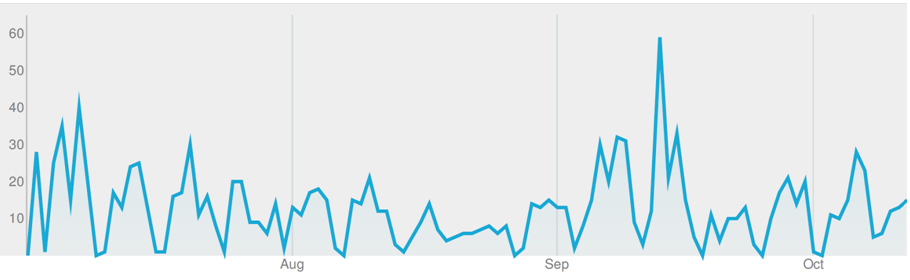
\includegraphics[scale=0.4]{Images/NUVI_time_distribution.png}
 \caption{Time distribution of the mentions of HPC profiles on Twitter between 1st July and 12th October 2017. The plot was created with the Twitter Analytics Tool NUVI.}
 \label{NUVI_time_distribution}
 \end{center}
\end{figure}

\subsubsection{Overview}
Monitored mentions sum up to 1323. The time distribution of the mentions is shown in figure \ref{NUVI_time_distribution}. The peak of conversation (59 mentions) happened on 12th September 2017. During the peak, the most frequently used keywords were filippo mantovani, workshop, server cpu, prototype and processors. An overview of the topics treated in the monitored mentions is provided in figure \ref{HPC_word_burst}. The figure is based on the 1005 mentions which came across 485 major categories over the monitored time. The list of most shared words is in table \ref{Most_shared_words}.

\begin{table}[t]
 \begin{center}
 %{\scriptsize
  \begin{tabular}{cccc}
   \hline 
   \hline
   Shared word & Mentions & Fraction of total mentions \\ 
   \hline
   \hline
   amp & 22 & 2.2\% \\
   project & 18 & 1.8\% \\
   supercomputer & 16 & 1.6\% \\
   application & 15 & 1.5\% \\
   etp4h & 14 & 1.4\% \\
   compute & 11 & 1.1\% \\
   \hline
   \hline
  \end{tabular}
 %} 
 \end{center} 
 \caption{List of the most shared words in the 1005 mentions of the HPC profiles which came across the 485 major categories considered by the Twitter Analytics Tool NUVI. The second and third columns list the amount of mentions in which the considered word was shared and the percentage of the considered mentions. The 1005 mentions are a subset of the 1323 monitored with NUVI between 1st July and 12th October 2017.}
\label{Most_shared_words} 
\end{table}

\subsubsection{Virality of the mentions}
Reach and spread together give an estimate of the potential audience which came across with the tweeted content. The reach is calculated as the sum of the followers of the accounts mentioning the analysed keyword. The spread is defined as the sum of the followers of the accounts which retweeted or shared the posts with the mention. Figure \ref{HPC_Most_reach_spread_popular} shows the mentions with the largest reach and spread, as well as the most popular one. 

\begin{figure}[H] 
 \begin{center}
 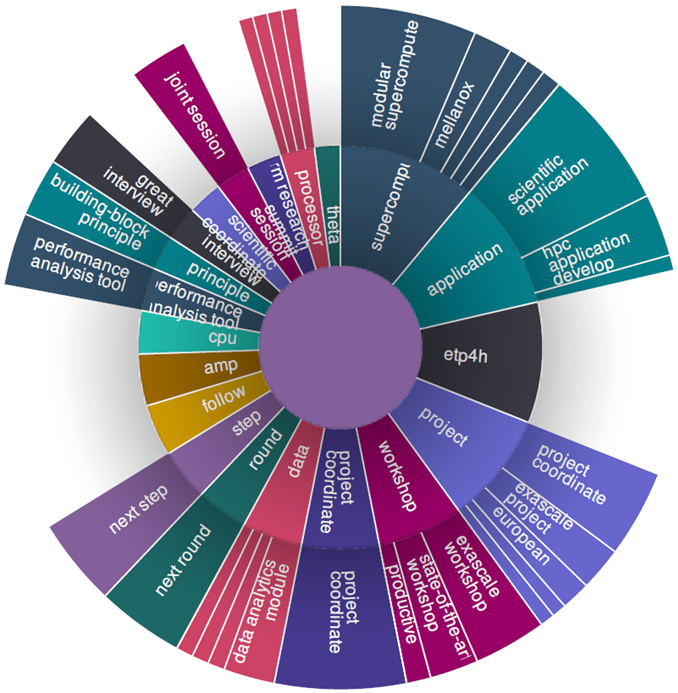
\includegraphics[scale=0.5]{Images/HPC_word_burst.png}
 \caption{Word burst of the mentions of HPC profiles monitored between 1st July and 12th October 2017 on Twitter. The figure is based on the 1005 mentions (out of 1323) which triggered 485 major categories. The analysis was performed with the Twitter Analytics Tool NUVI.}
 \label{HPC_word_burst}
 \end{center}
\end{figure}

\begin{figure}[!t] 
 \begin{center}
 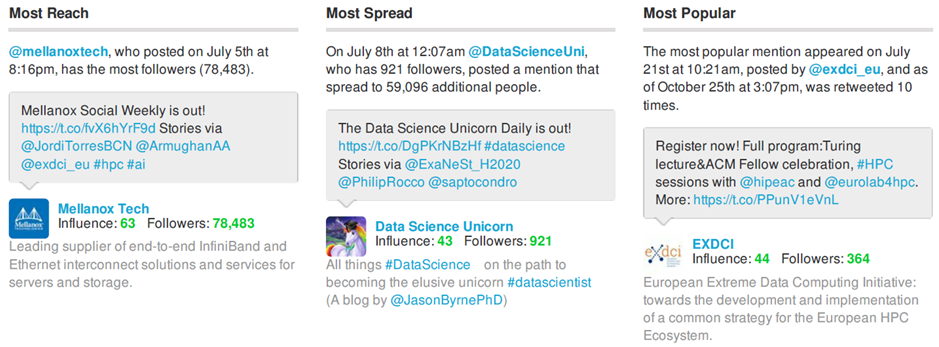
\includegraphics[scale=0.41]{Images/HPC_Most_reach_spread_popular.png}
 \caption{Three of the 1323 mentions of HPC projects on Twitter monitored between 1st July and 12th October 2017: the mentions with the largest reach, the largest spread and the most popular one. Data were collected with the Twitter Analytics Tool NUVI.}
 \label{HPC_Most_reach_spread_popular}
 \end{center}
\end{figure}

Out of the 1323 monitored mentions, 637 were original posts. These had all together the potential of reaching an audience of 172 720 users. A total amount of 686 reshares was made by 116 unique profiles. The reshares spread the mentions to 233 974 users. The ratio between reach and spread defines the viral coefficient. For the monitored mentions and over the investigated period, it value is equal to 1.4, see figure \ref{HPC_viral_coefficient}. As the viral coefficient is larger than one, monitored mentions can be considered extremely viral. 

\begin{figure}[H] 
 \begin{center}
 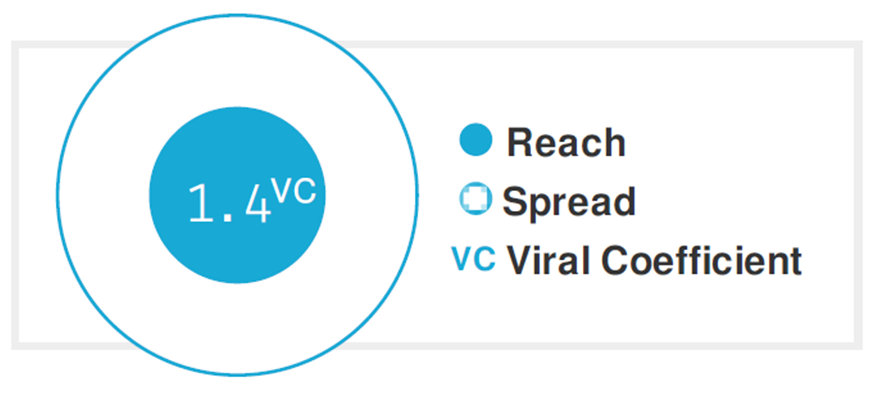
\includegraphics[scale=0.2]{Images/HPC_viral_coefficient.png}
 \caption{Graphic comparison of the reach (172 720 users) and spread (233 974 users) of the mentions of HPC projects on Twitter between 1st July and 12th October 2017. The viral coefficient is defined as the ratio between spread and reach. Data were collected with the Twitter Analytics Tool NUVI.}
 \label{HPC_viral_coefficient}
 \end{center}
\end{figure}

\section{Projects with most viral mentions}
Results in section \ref{Mentions_of_HPC_profiles} refer to the whole set of mentions of HPC monitored over the analysed weeks. The data breakdown for each single project is summarised in table \ref{HPC_viral_coefficients}. It is worth noting that the values of reach, spread and viral coefficient vary significantly among HPC projects. The medians of the three variables are 4056, 4836 and 0.7, respectively.      

Seven out of seventeen projects have been mentioned in viral conversations (i.e., with viral coefficients larger than unity). The projects with the largest viral coefficients are ECOSCALE (41.2), NEXTGenIO (13.5) and EuroLab-4-HPC (6.9). It is worth noting the following: \textit{i}) the largest viral coefficient of ECOSCALE originates from the low number of mentions of the project; \textit{ii}) EuroLab-4-HPC is mentioned in viral posts although it had posted no tweets by the time of writing, see table \ref{HPC_Twitter_activity}; \textit{iii}) with the exception of EXDCI, the most influential projects identified in section \ref{Most_influential_projects} are all mentioned in viral conversations.

\section{Chapter summary}
In this chapter, the following items have been discussed:

\begin{enumerate}
 \item The activity of HPC projects on Twitter ranges between roughly one tweet every three months and three tweets every second day. The median calculated over all HPC Twitter profile is approximately one tweet per week. HPC projects perform well in terms of profile's tweets retweeted by other and shared links. The medians of the two statistics are comparable to the corresponding values calculated for the Twitter account of the FET funding programme.
 \item The most influential HPC projects on Twitter were found to be ExaFLOW, EXDCI, Mont-Blanc 3 and NEXTGenIO. In general, HPC influential initiatives are identified by a number of followers and a ratio followers/following larger than $\approx 100$ and $\approx 2$, respectively. 
 \item The mentions of HPC projects on Twitter were found to be viral over a period of three and a half months. The result indicates that the Twitter community interested in FET HPC initiatives is large. Thus, the decision of the vast majority of HPC projects to consider Twitter for their communication campaign is correct.
 \item In general, the most influential HPC projects are also those mentioned in the most viral conversations.    
\end{enumerate}  


\begin{table}[t]
 \begin{center}
 {\scriptsize
  \begin{tabular}{cccc}
   \hline 
   \hline
   Project & Reach & Spread & Viral coefficient \\ 
   \hline
   \hline
   ALLScale & 48 & 0 & 0.0 \\
   ANTAREX & 202 & 9 & 0.0 \\
   COMPAT & 13 286 & 112 & 0.0 \\
   DEEP-EST & 11 759 & 6 988 & 0.6 \\
   ECOSCALE & 55 & 2 268 & 41.2 \\
   EuroLab-4-HPC & 2 135 & 14 679 & 6.9 \\
   ExaFLOW & 18 366 & 28 311 & 1.5 \\
   ExaNeSt & 18 109 & 62 259 & 3.4  \\
   ExaNoDe & 6 559 & 4 470 & 0.7 \\
   EXDCI & 111 534 & 23 082 & 0.2 \\
   EXTRA & 216 & 24 & 0.1 \\
   INTERTWINE & 7 436 & 6 673 & 0.9 \\
   MANGO & 1 360 & 162 & 0.1 \\
   Mont-Blanc 3 & 30 362 & 58 782 & 1.9 \\
   NEXTGenIO & 4 056 & 53 838 & 13.5 \\
   READEX & 117 & 0 & 0.0 \\
   SAGE & 1 537 & 4 836 & 3.1 \\ 
   \hline
   \hline
  \end{tabular}
 } 
 \end{center} 
 \caption{Reach, spread and viral coefficient of the mentions of each HPC project on Twitter between 1st July and 12th October 2017. The viral coefficient is defined as the ratio between spread and reach. Data were collected with the Twitter Analytics Tool NUVI.}
\label{HPC_viral_coefficients} 
\end{table}
 \chapter{The QT communication potential on Twitter} 
Lorem ipsum dolor sit amet, consectetur adipisci elit, sed eiusmod tempor incidunt ut labore et dolore magna aliqua. Ut enim ad minim veniam, quis nostrum exercitationem ullam corporis suscipit laboriosam, nisi ut aliquid ex ea commodi consequatur. Quis aute iure reprehenderit in voluptate velit esse cillum dolore eu fugiat nulla pariatur. Excepteur sint obcaecat cupiditat non proident, sunt in culpa qui officia deserunt mollit anim id est laborum.

Data shown in this chapter was collected with the Twitter Analytics Tool Twitonomy. 

\section{Hashtag performance}
Two hashtags were monitored to assess of the reach potential of FET projects on QTs. These were \#quantumcomputing and the application of the AND logic operator to \#quantum and \#technology. 

Both analyses covered two periods of time. For \#quantumcomputing, the two periods were from 7th to 14th and from 20th to 25th October 2017, respectively. Those for the combination \#quantum AND \#technology spanned the time intervals between 4th and 14th and between 15th and 25th October 2017. The time periods were chosen randomly and based on the day ranges available to Twitonomy for the considered volume of tweets. Different choices of the time periods would not change significantly the estimates presented in this chapter.  

The distribution of the number of Tweets presenting the hashtags \#quantumcomputing and the combination \#quantum AND \#technology over the considered periods are shown in figures \ref{First-SecondSearch_QuantumComputing.png} and \ref{First-SecondSearch_QuantumTechnology.png}. The plots show that, typically, hundreds of tweets with the hashtag \#quantumcomputing are posted daily, whereas few show both hashtags \#quantum and \#technology. 

The potential reach of FET projects on QTs is summarised by data in Tables \ref{Summary_QuantumComputing-Technology}. 

\begin{table}[t]
 \begin{center}
 
  \begin{tabular}{ccccc}
   \hline 
   \hline
   Time period & Tweets & Users & Potential Reach \\ 
   \hline
   \hline
   7 - 14 Oct 2017 & 1 928 & 1 270 & 9 392 166  \\
   20 - 25 Oct 2017 & 2 563 & 1 738 & 10 604 445  \\
   \hline
   \hline
  \end{tabular}

  \bigskip

  \begin{tabular}{ccccc}
   \hline 
   \hline
   Time period & Tweets & Users & Potential Reach \\ 
   \hline
   \hline
   4 - 14 Oct 2017 & 79 & 75 & 280 849  \\
   15 - 25 Oct 2017 & 36 & 28 & 85 123  \\
   \hline
   \hline
  \end{tabular}
 \end{center} 
 \caption{Summary of the Twitter analytics for the hashtag combination \#quantum AND \#technology over the two monitored time periods. The potential reach is defined as the total aggregate number of followers of the people who mentioned the considered keyword in their tweets.}
\label{Summary_QuantumComputing-Technology} 
\end{table}    

\begin{figure}
 \centering
 \begin{subfigure}[b]{0.9\textwidth}
   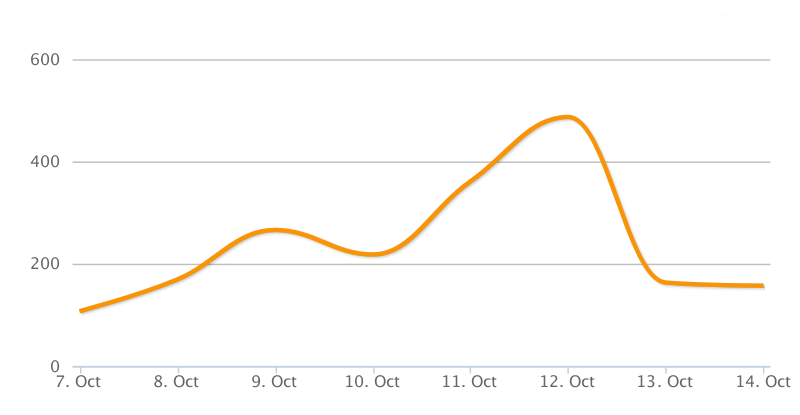
\includegraphics[width=1\linewidth]{Images/FirstSearch_QuantumComputing.png}
   \caption{} 
 \end{subfigure}

 \begin{subfigure}[b]{0.9\textwidth}
   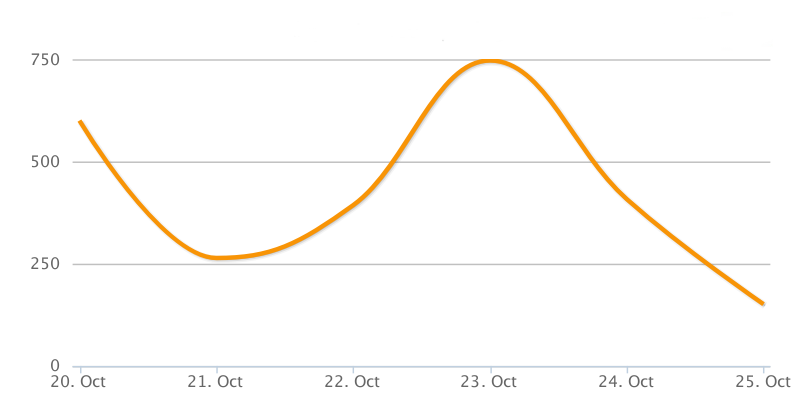
\includegraphics[width=1\linewidth]{Images/SecondSearch_QuantumComputing.png}
   \caption{}
 \end{subfigure}
 \caption{(a) Number of tweets with hashtag \#quantumcomputing posted between 7th and 14th October 2017. (b) As for (a) but over the time period between 20th and 25th October 2017.} 
 \label{First-SecondSearch_QuantumComputing.png}
\end{figure}

\begin{figure}
 \centering
 \begin{subfigure}[b]{0.9\textwidth}
   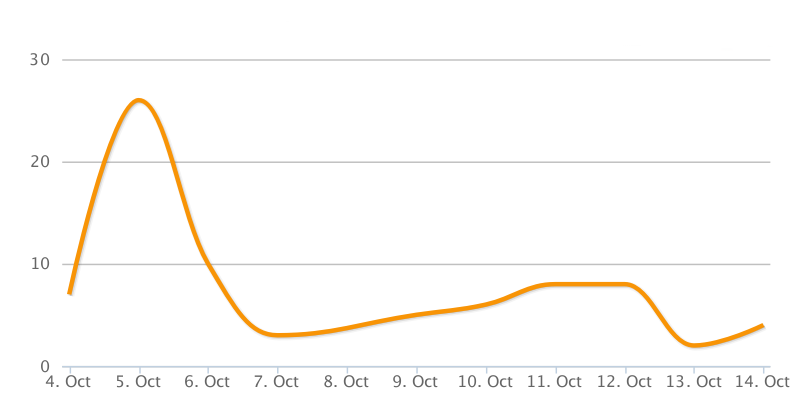
\includegraphics[width=1\linewidth]{Images/FirstSearch_QuantumTechnology.png}
   \caption{} 
 \end{subfigure}

 \begin{subfigure}[b]{0.9\textwidth}
   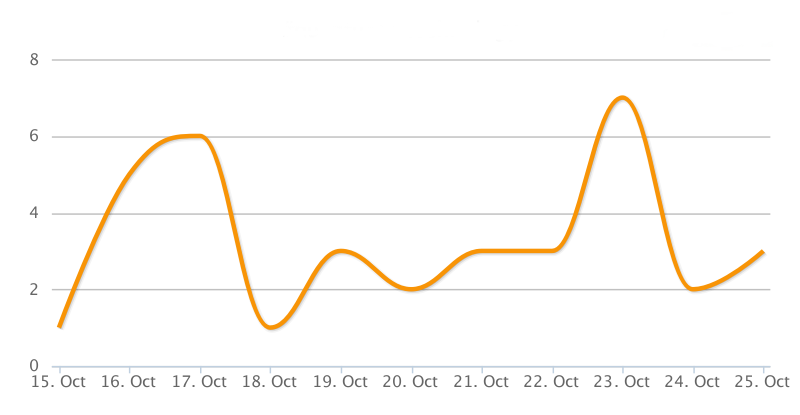
\includegraphics[width=1\linewidth]{Images/SecondSearch_QuantumTechnology.png}
   \caption{}
 \end{subfigure}
 \caption{(a) Number of tweets with hashtags \#quantum and \#technology posted between 4th and 14th October 2017. (b) As for (a) but over the time period between 15th and 25th October 2017.} 
 \label{First-SecondSearch_QuantumTechnology.png}
\end{figure}
 \chapter*{Conclusions}
This thesis focused on the online aspects of the communication campaigns designed by FET research projects. The results indicate that FET initiatives do consider social media as an opportunity to reach stakeholders and the general public. Nevertheless, the use of online channels is not uniform across disparate FET investigation lines.  

One example is offered by HPC and QT research projects. The two classes face similar communication challenges and pursue partially overlapping objectives (although the strategies to achieve them are very different). Despite such similarities, the approaches followed by HPC and QT projects are opposite. On one hand, HPC initiatives make an effective use of popular social media such as Twitter and Facebook. On the other hand, QT projects do not base their communication efforts on online platforms. In particular, they disregard Twitter.  

The motivation for the different behaviour lies probably in the fact that the development of QTs is still in the initial phase. It is not known yet whether this effort will indeed be successful. Hence, applications to society are not to be expected in the near future. 

Nevertheless, the limited use of social media made by QT projects may reduce the societal uptake of this investigation line. The potential reach of QT initiatives was estimated to be comparable to the online community interested in HPC projects, which consists of hundreds of thousands of users. Expanding the community coming in contact with QT research would draw attention on this potentially groundbreaking scientific frontier and may attract funding.

A more active use of social media may be expected from the FET Flagship initiative on QTs. This is one of the major investigation efforts ever undertaken by the European Union and will be launched in 2018. However, a strong presence of QT projects on social platforms prior to the beginning of the flagship initiative may have \textit{i}) provided useful hints and guidelines on how to best design an effective QT communication strategy, and \textit{ii}) contributed to building a preexisting engaged community.
 \addcontentsline{toc}{chapter}{Conclusions}
 
 \appendix
 \chapter{List of FET projects} \label{List_of_FET_projects}
Lorem ipsum dolor sit amet, consectetur adipisci elit, sed eiusmod tempor incidunt ut labore et dolore magna aliqua. Ut enim ad minim veniam, quis nostrum exercitationem ullam corporis suscipit laboriosam, nisi ut aliquid ex ea commodi consequatur. Quis aute iure reprehenderit in voluptate velit esse cillum dolore eu fugiat nulla pariatur. Excepteur sint obcaecat cupiditat non proident, sunt in culpa qui officia deserunt mollit anim id est laborum.

\afterpage{
 \clearpage% Flush earlier floats (otherwise order might not be correct)
 \thispagestyle{empty}% empty page style
   \begin{landscape}% Landscape page
   %\begin{center}
    \begin{adjustwidth}{-3cm}{}
    {\tiny
    \begin{tabular}{cccccccc}
	  \hline 
  	  \hline
       Project & Start date & End date & Total fund & EU fund & Website & Twitter & Facebook \\ 
       \hline
       \hline
       ABIOMATER & 01/11/2015 & 31/10/2018 & 2 978 882 & 2 978 882 & blogs.exeter.ac.uk/abiomater & @abiomater & \\		
       A-LEAF & 01/01/2017 & 31/12/2020 & 7 980 861 & 7 980 861 & a-leaf.eu & @aleaf\textunderscore h2020 & aleaf.h2020 \\
       ALLScale & 01/10/2015 & 30/09/2018 & 3 366 196 & 3 366 196 & allscale.eu/home &	@AllScaleEurope & AllScaleProject \\
       AMECRYS & 01/10/2016 & 30/09/2020 & 3 533 813 & 3 533 813 & amecrys-project.eu & @amecrysproject & amecrysproject \\
       AQuS & 01/01/2015 & 31/12/2017 & 2 000 500 & 2 000 500 & kip.uni-heidelberg.de/aqus & & \\
       BREAKBEN	& 01/01/2016 & 31/12/2018 & 3 998 793 & 3 998 793 & breakben.eu & @BREAKBENeu & \\
       CASEK & 01/04/2017 & 30/09/2018 & 100 000 & 100 000 & casek.eu & & \\ 	
       ChipScope & 01/01/2017 & 31/12/2020 & 3 759 790 & 3 759 790 & chipscope.eu & @ChipScope\textunderscore EU & chipscope \\
       CHROMAVISION	& 01/06/2015 & 31/05/2019 & 3 567 025 & 3 567 025 & chromavision.eu & & \\
       CResPace	& 01/01/2017 & 31/12/2021 & 4 944 347 & 4 944 347 & crespace.eu & & \\
       DEEP-EST & 01/07/2017 & 30/06/2020 & 15 873 341 & 14 998 342 & deep-projects.eu &	@DEEPprojects & \\
       DIACAT & 01/07/2015 & 30/06/2019 & 3 872 981 & 3 872 981 & diacat.eu & @DIACAT\textunderscore EU & \\
       DISCOVERER &	01/01/2017 & 31/03/2021 & 5 726 750 & 5 726 750 & discoverer.space & @DISCOVERER\textunderscore EU & \\
       DMS & 01/04/2017 & 30/09/2018 & 100 000 & 100 000 & & & \\
       D-Noise & 01/05/2017 & 31/10/2018 & 130 937 & 100 000 & d-noise-fet.eu & & \\
       DREAM & 01/01/2015 & 31/12/2018 & 2 784 240 & 2 730 241 & robotsthatdream.eu & @robotsthatdream & \\
       ECOSCALE	& 01/10/2015 & 30/09/2018 & 4 237 397 & 4 237 397 & ecoscale.eu & @ECOSCALE\textunderscore H2020 &	\\	
       ENTIMENT	& 01/07/2017 & 31/12/2018 & 100 000 & 100 000 & & & \\
       EuroEXA & 01/09/2017 & 28/02/2021 & 19 949 022 & 19 949 022 & & & \\
       ESCAPE & 01/10/2015 & 30/09/2018 & 3 977 952 & 3 977 952 & hpc-escape.eu & & \\
       EuroLab-4-HPC & 01/09/2015 & 31/08/2017 & 1 489 981 & 1 489 981 & eurolab4hpc.eu & @eurolab4hpc & \\
       ExaFLOW & 01/10/2015 & 30/09/2018 & 3 312 235 & 3 312 235 & exaflow-project.eu & @exaflowproject & \\			
       ExaNeSt & 01/12/2015 & 30/11/2018 & 8 442 547 & 8 442 547 & exanest.eu & @exanest\textunderscore h2020 & Exanest\textunderscore h2020-282450078883797 \\
       ExaNoDe & 01/10/2015 & 30/09/2018 & 8 629 247 & 8 629 247 & exanode.eu & @ExanodeProject & Exanode-1669383456699997 \\
       ExCAPE &	01/09/2015 & 31/08/2018 & 3 910 140 & 3 910 140 & excape-h2020.eu & & \\
       EXDCI & 01/09/2015 & 28/02/2018 & 2 551 875 & 2 551 875 & exdci.eu & @exdci\textunderscore eu & \\
       FEMTOTERABYTE & 01/03/2017 & 29/02/2020 & 3 712 832 & 3 712 832 & physics.gu.se/english/research/femtoterabyte & & \\
       FLAG-ERA II & 01/12/2016 & 30/11/2021 & 18 341 250 & 6 052 612 & flagera.eu & & flagera \\
       flora robotica &	01/04/2015 & 31/3/2019 & 3 641 781 & 3 641 781 & florarobotica.eu & @florarobotica & florarobotica \\
       GOAL-Robots & 01/11/2016 & 31/10/2020 & 3 481 875 & 3 481 875 & goal-robots.eu & & \\       
       GRACeFUL & 01/02/2015 & 31/01/2018 & 2 404 943 & 2 404 943 & graceful-project.eu &  @gracefulproject & \\
       GrapheneCore1 & 01/04/2016 &	31/03/2018 &	89 000 000 & 89 000 000	& graphene-flagship.eu & @GrapheneCA	& GrapheneFlagship \\
       greenFLASH & 01/10/2015 & 30/09/2018 & 3 760 793 & 3 760 793 & greenflash-h2020.eu & & \\
       HELENIC-REF & 01/06/2015 & 31/05/2018 & 2 578 386 & 2 578 386 & helenic-ref.eu & & \\
       INTERLACE & 01/05/2017 &	31/10/2018 & 99 978 & 99 978 & & & \\										
       \hline
       \hline
    \end{tabular}
    }
    \end{adjustwidth}
   %\end{center}
   \end{landscape}
 \clearpage
}

\newpage

\afterpage{
 \clearpage% Flush earlier floats (otherwise order might not be correct)
 \thispagestyle{empty}% empty page style
   \begin{landscape}% Landscape page
   %\begin{center}
    \begin{adjustwidth}{-3.5cm}{}
    {\tiny
    \begin{tabular}{cccccccc}
	  \hline 
  	  \hline
       Project & Start date & End date & Total fund & EU fund & Website & Twitter & Facebook \\ 
       \hline
       \hline
       INTERTWINE & 01/10/2015 & 30/09/2018 & 3 861 400 & 3 861 400 & intertwine-project.eu & @intertwine\textunderscore eu & \\
       LiRichFCC & 01/10/2016 & 30/09/2019 & 4 114 753 & 4 114 753 & lirichfcc.eu & & \\
       Lumiblast & 01/10/2016 & 31/03/2021 & 3 031 375 & 3 031 375 & lumiblast.eu & & \\
       MAGENTA & 01/01/2017 & 31/12/2020 & 4 999 778 & 4 999 777 & magenta-h2020.eu & & \\
       MAGicSky & 01/09/2015 & 31/08/2018 & 3 396 439 & 3 396 439 & magicsky-fet.eu & @magicskyf & \\
       MAGNEURON & 01/01/2016 &	31/12/2019 & 3 473 026 & 3 473 026 & magneuron.eu & & \\
       Microflusa & 01/09/2015 & 31/08/2019 & 3 027 637 & 3 027 637 & microflusa-project.eu & & \\
       MIR-BOSE & 01/01/2017 & 31/12/2020 & 3 786 160 & 3 786 160 & mir-bose.eu & & \\
       MRG-GRammar & 01/08/2015 & 31/07/2018 & 3 999 661 & 3 999 661 & mrg-grammar.eu & @MrgGrammar\textunderscore proj & mrggrammar \\
       NanoSmell & 01/09/2015 &	31/08/2019 & 3 979 069 & 3 979 069 & nanosmell.org & & \\
       Neurofibres & 01/01/2017 & 31/12/2020 & 5 888 491 & 5 094 120 & neurofibres.eu & @neurofibres & \\
       nuClock & 01/06/2015	& 31/05/2019 & 3 970 327 & 3 970 327 & nuclock.eu & & nuclock.eu \\
       PHENOMEN	& 01/09/2016 & 31/08/2019 & 2 915 886 & 2 915 886 & phenomen-project.eu & & \\ 
       QCUMbER & 01/09/2015	& 31/08/2018 & 3 219 721 & 3 219 721 & qcumber.eu & & \\
       Qdet & 01/05/2017 & 31/10/2018 & 100 000 & 100 000 & & & \\
       QuantERA	& 01/11/2016 & 31/10/2021 & 40 464 570 & 11 510 008	& quantera.eu & & QuanteraCoFund \\
       QUCHIP & 01/03/2015 & 28/02/2018 & 2 681 713 & 2 681 713 & quchip.eu & & \\
       QUIC & 01/03/2015 & 28/02/2019 & 2 774 375 & 2 386 875 & quic-project.eu & & \\
       QuProCS & 01/04/2015 & 31/3/2018 & 2 268 746 & 2 268 746 & quprocs.eu & & \\
       QUSMI & 01/05/2017 & 31/10/2018 & 96 462 & 96 462 & nvision-imaging.com & & \\	
       RYSQ & 01/03/2015 & 28/02/2018 & 4 695 000 & 4 383 000 & qurope.eu/projects/rysq & & \\
       SC-square & 01/07/2016 & 31/8/2018 & 499 603 & 499 603 & sc-square.org & & \\
       SENSE & 01/09/2016 &	31/08/2019 & 886 500	& 886 500 & sense-pro.org & @senselowlight & \\
       SensAgain & 01/09/2017 & 28/02/2019 & 99 912 & 99 912 & & & \\
       SiLAS & 01/01/2017 & 31/12/2020 & 3 985 417 & 3 985 417 & silasproject.eu & & \\		
       SmartNurse & 01/05/2017 & 31/10/2018 & 100 000 & 100 000 & & & \\
       socSMCs & 01/01/2015 & 31/12/2018 & 3 778 125 & 3 778 125 & socsmcs.eu & @socSMCs & \\		
       subCULTron & 01/04/2015 & 31/03/2019 & 3 987 650 & 3 987 650 & subcultron.eu & @subCULTron & \\
       2D-INK & 01/01/2016 & 31/12/2018 & 2 962 661	& 2 962 661 & 2d-ink.eu & @2D\textunderscore INK & 2D-INK-1419976004971237 \\
       ULTRACHIRAL & 01/01/2017 & 31/12/2020 & 3 999 250 & 3 999 250 & ultrachiral.iesl.forth.gr & @ultrachiral & \\	
       VISORSURF & 01/01/2017 & 30/6/2020 & 5 748 000 & 5 748 000 & visorsurf.eu & @VisorSurf & VisorSurf/?ref=br\textunderscore rs \\
       WASPSNEST & 01/06/2017 & 31/05/2018 & 99 775 & 99 775 & fp7wasps.org/en/ & & \\			
       WhiteRabbit & 01/04/2017 & 31/07/2018 & 99 750 & 99 750 & & & \\	
       \hline
       \hline
    \end{tabular}
    }
    \end{adjustwidth}
   %\end{center}
   \end{landscape}
 \clearpage
}
 \chapter{Specific lists of FET projects} \label{Specific_lists_of_FET_projects}
Disparate groups of projects in Appendix \ref{List_of_FET_projects} were considered in this thesis. The motivations for the identification of the groups are outlined in section \ref{Data_set}. The projects in each of the groups are listed below.

\section{Disregarded projects}
The following groups of projects were not considered for the analyses preseted in this thesis:

\subsubsection{Flagship projects}
GrapheneCore1 and HBP SGA1.

\subsubsection{Launchpad projects}
aPad, CASEK, CF-Web, D-Noise, DMS, ENTIMENT, I2C8, INTERLACE, PhySense, Qdet, QUSMI, ROMA, SensAgain, SmartNurse, WASPSNEST and WhiteRabbit.

\subsubsection{Started after 1st February 2017}
CATCH-U-DNA, EuroEXA and FEMTOTERABYTE. The DEEP-EST project was also launched after 1st February 2017. Nevertheless, it was considered for the analysis as it had already activated several communication channels by the time of writing.

\section{Investigated classes}
This thesis presents a comparison of the use of online communication channels made by projects active in high-performing computing and in the development of quantum technologies. The projects in the two classes are listed below. 

\subsubsection{High performing computing (HPC)}
ALLScale, ANTAREX, ComPat, DEEP-EST, ECOSCALE, ESCAPE, EuroLab-4-HPC, ExaFLOW, ExaHyPE, ExaNeSt, ExaNoDe, ExCAPE, EXDCI, EXTRA, greenFLASH, INTERTWINE, MANGO, Mont-Blanc 3, NEXTGenIO, NLAFET, READEX and SAGE. The  EuroEXA project was not considered as it was launched after 1st February 2017, see above.

\subsubsection{Quantum technologies (QT)}
AQuS, MaQSens, NanOQTech, QCUMbER, QuantERA, QUCHIP, QUIC, QuProCS, RYSQ and ULTRAQCL. The QUSMI e Qdet projects were not considered as they were launched after 1st February 2017, see above.
 
 \bibliography{Thesis_chapters/Bibliography}
 \bibliographystyle{IEEEtran}
 \addcontentsline{toc}{chapter}{References}

\end{document}